\documentclass[10pt, twocolumn]{article}

% ------ Geometry ------------------------------------------------------------------------------------------------------------------------------------------------------------------------------------------------------
\usepackage[top=1in, bottom=1in, left=0.75in, right=0.75in,
            columnsep=0.25in]{geometry}

% ------ Core packages ---------------------------------------------------------------------------------------------------------------------------------------------------------------------------------------
% newtxtext/newtxmath give Times-compatible text AND math with working bold.
% (The legacy `times` package silently drops to regular weight under some
%  engines, leaving section and run-in headers un-bolded.)
\usepackage{amsmath, amsthm}
\usepackage{newtxtext,newtxmath}
\usepackage{microtype}
\usepackage{graphicx}
\graphicspath{{../}{./}}
\usepackage{booktabs}
\usepackage{multirow}
\usepackage{array}
\usepackage{xcolor}
\usepackage{url}
\usepackage{caption}
\usepackage{subcaption}
\usepackage{enumitem}
\usepackage{algorithm}
\usepackage{algpseudocode}
\usepackage[square,numbers,sort&compress]{natbib}
\usepackage[colorlinks=true, linkcolor=NavyBlue, citecolor=NavyBlue,
            urlcolor=NavyBlue]{hyperref}
\definecolor{NavyBlue}{rgb}{0.0,0.13,0.4}

% ------ Abstract spanning both columns ------------------------------------------------------------------------------------------------------------------------------------
\usepackage{abstract}
\renewcommand{\abstractnamefont}{\normalfont\bfseries}
\renewcommand{\abstracttextfont}{\normalfont\small}

% ------ Section formatting ------------------------------------------------------------------------------------------------------------------------------------------------------------------------
\usepackage{titlesec}
\titleformat{\section}{\normalfont\large\bfseries}{\thesection}{1em}{}
\titleformat{\subsection}{\normalfont\normalsize\bfseries}{\thesubsection}{1em}{}
\titleformat{\paragraph}[runin]{\normalfont\normalsize\bfseries}{}{0em}{}[.\enspace]
\setlength{\parskip}{2pt}

% ------ Title block ---------------------------------------------------------------------------------------------------------------------------------------------------------------------------------------------
\title{%
  \vspace{-1.5em}%
  \large\textbf{The Small Librarian: Characterizing and Repairing\\[2pt]
  Memory Rot in Strictly On-Device Small-Model Agents}%
  \vspace{-0.5em}%
}

\author{%
  \normalsize Prashant Mudgal \\[-2pt]
  \small Nagarro \\[-2pt]
  \small \texttt{prashant.mudgal@nagarro.com} \\[-2pt]
  \small \texttt{prashantmdgl9@gmail.com}
}

\date{\small\today}

% ------ Theorem environments ------------------------------------------------------------------------------------------------------------------------------------------------------------------
\newtheorem{definition}{Definition}
\newtheorem{observation}{Observation}

\begin{document}

% ------ Title + abstract (full width) ---------------------------------------------------------------------------------------------------------------------------------------
\twocolumn[{%
  \maketitle
  \begin{onecolabstract}
On-device language model agents require persistent memory to sustain coherent
long-horizon interactions, yet the memory management capability of small models
(3--8B parameters) has not been systematically studied.
We identify and characterize \emph{memory rot}: the progressive accumulation of
stale, contradictory, and redundant facts caused by small models' near-complete
failure to fire \textsc{update} and \textsc{delete} memory operations.
On a controlled 80-turn injection stream with ground-truth operation labels,
naive LLM-driven memory management achieves only 0--31\% \textsc{update}
recall and 0--50\% \textsc{delete} recall across five on-device models.
We propose \textbf{The Small Librarian}, a lightweight framework that replaces
probabilistic operation routing with two deterministic mechanisms:
\emph{typed slots} (one store entry per fact key, eliminating model judgment for
\textsc{update}) and \emph{deletion signals} (rule-based keyword detection for
\textsc{delete}).
Typed slots alone raise \textsc{update} recall to 27--100\% across four of
five models, a mean gain of 61 percentage points, without additional
parameters or API calls.
A four-condition ablation with 95\% Wilson confidence intervals reveals that
deletion signals further improve \textsc{delete} recall but introduce
false-positive erasures that partially offset downstream QA gains,
motivating periodic compaction as a safety net for key fragmentation.
All components run strictly on-device with open-weight models and no paid APIs.
  \end{onecolabstract}
  \vspace{1em}
}]

%% ---------------------------------------------------------------------------------------------------------------------------------------------------------------------------------------------------------------------------------------
\section{Introduction}
\label{sec:intro}

Memory is the foundation of any useful personal agent, and user context is
fundamentally dynamic. Facts change, beliefs evolve, and prior information
is sometimes explicitly revoked. A reliable memory subsystem must handle all
three operations correctly: \emph{adding} new knowledge, \emph{updating}
what has changed, and \emph{deleting} what no longer holds. Failing even one
of these causes the agent's world-model to drift from reality, accumulating
contradictions that compound silently across sessions.

Large proprietary models handle this competently when memory is framed as a
structured task~\cite{packer2023memgpt}.
Small on-device models (3--8B parameters) face a fundamentally different
regime: limited context windows, weaker instruction following, reduced
capacity for multi-step reasoning, and sensitivity to prompt formatting.
Whether they can serve as their own memory managers, reliably classifying and
routing memory operations under a strict on-device constraint, is an open
empirical question with significant practical consequences.
Millions of edge devices run small open-weight models today; the quality of
their memory subsystems directly determines whether they can serve as useful
personal assistants over long horizons.

We answer this question with a controlled diagnostic: a synthetic 80-turn
conversation stream where each turn carries a ground-truth memory operation
label (\textsc{add}, \textsc{update}, \textsc{delete}, or \textsc{noop}).
Unlike downstream QA evaluation, this lets us measure per-operation recall
and precision directly, isolating exactly where small models fail.

\paragraph{Key finding: memory rot}
Across five on-device models (Qwen3-4B/8B, LLaMA-3.2-3B, LLaMA-3.1-8B,
and Qwen2.5-7B), naive LLM-driven memory management virtually never fires
\textsc{update}: mean recall is only 10\% (range 0--31\%).
\textsc{delete} recall is similarly poor at 26\% (range 0--50\%).
Two models collapse entirely to \textsc{noop}, firing no operations regardless
of turn content.
Both behaviors corrupt the store in complementary ways: indiscriminate
\textsc{add} bloats it with superseded, contradictory versions of a fact,
while \textsc{noop} collapse leaves it empty and missing facts entirely.
Either way the store drifts from the true state of the world, and that
divergence grows with every turn.
We call this failure mode \emph{memory rot}, by analogy with code rot:
not a catastrophic failure, but a slow accumulation of entropy that eventually
makes the system unreliable.

\paragraph{Why memory rot is hard to detect}
A critical methodological contribution of this work is demonstrating that
downstream QA metrics \emph{mask} memory rot.
We find that RAG over raw conversation turns consistently outperforms an
LLM-managed memory store (60--75\% vs.\ 10--25\% QA EM on LongMemEval-S).
This counterintuitive result occurs because a rotten store actively
misleads the retrieval step: contradictory entries compete, and the LLM
retrieves stale facts.
Without per-operation ground-truth labels, this failure mode looks like a
``QA difficulty'' rather than a ``memory management failure.''

\paragraph{The Small Librarian}
We propose a framework that addresses memory rot without increasing model
size or adding external API calls.
The core insight is that \textsc{update} failures are not failures of
comprehension: small models correctly identify \emph{what} the new fact
is, but fail at \emph{routing}. The model assigns \textsc{add} instead
of \textsc{update} because it does not reliably recognize when a new fact
supersedes an existing one.
Typed slots eliminate the routing decision entirely.
Deletion signals handle \textsc{delete} via curated keyword matching,
bypassing model judgment for a class of operations that follow predictable
surface patterns.

\paragraph{Contributions}
\begin{enumerate}[leftmargin=*, itemsep=1pt, topsep=2pt]
  \item We introduce \emph{memory rot} as a named, measurable failure mode
    and provide the first controlled characterization of per-operation
    recall/precision for small on-device memory managers~(\S\ref{sec:phase2}).
  \item We propose The Small Librarian with typed slots and deletion signals,
    both fully on-device and parameter-free~(\S\ref{sec:framework}).
  \item We conduct a four-condition ablation with 95\% Wilson confidence
    intervals, isolating the independent contribution of each mechanism and
    revealing a precision--recall tradeoff in deletion signals~(\S\ref{sec:ablation}).
\end{enumerate}

%% ---------------------------------------------------------------------------------------------------------------------------------------------------------------------------------------------------------------------------------------
\section{Related Work}
\label{sec:related}

\paragraph{Memory-augmented language models}
Weston et al.~\cite{weston2014memory} and Graves et al.~\cite{graves2014neural}
introduced external memory as a differentiable component of neural networks.
More recently, MemGPT~\cite{packer2023memgpt} frames LLM memory management
as an operating system problem, with the LLM acting as its own memory
controller.
LangChain Memory, Mem0, and similar frameworks operationalize this idea for
production agents.
Our work complements these by characterizing the failure modes that emerge
when the ``controller'' is a small on-device model rather than a capable
cloud LLM.

\paragraph{Long-context and retrieval-augmented QA}
LongMemEval~\cite{wu2024longmemeval} benchmarks chat assistants on long-term
interactive memory with sessions averaging tens of thousands of tokens.
LoCoMo~\cite{maharana2024evaluating} evaluates very long-term conversational
memory spanning months of interaction.
Both benchmarks measure downstream QA quality; neither isolates which
memory operations fail or why.
We introduce a complementary controlled injection stream that provides
operation-level ground truth, enabling mechanistic analysis.

\paragraph{RAG vs.\ structured memory}
Retrieval-augmented generation~\cite{lewis2020retrieval} retrieves relevant
documents at inference time without maintaining a structured memory store.
Prior work has shown RAG to be competitive with or superior to explicit
memory management in some settings~\cite{shi2023large}.
Our Phase~1 results on LongMemEval-S extend this finding to the small-model
regime: RAG over raw turns outperforms LLM-managed memory because memory
rot actively corrupts the store's signal.

\paragraph{On-device inference}
MLC-LLM, llama.cpp, and Ollama~\cite{ollama2024} enable deployment of
3--8B quantized models on consumer hardware with acceptable latency.
Recent work on quantization~\cite{dettmers2022gptq} and efficient
attention~\cite{dao2022flashattention} makes these models viable for
always-on agent deployment.
Memory management for such models has received little systematic attention.

\paragraph{Structured and typed memory for agents}
Several papers propose hierarchical or typed memory
stores~\cite{zhong2024memorybank,zhang2024survey}, and cognitive
architectures~\cite{anderson1983architecture} have long distinguished
episodic, semantic, and procedural memory.
To our knowledge, no prior work characterizes operation-level recall
for small models specifically, or proposes parameter-free mechanisms
targeting the \textsc{update}/\textsc{delete} failure modes we identify.

%% ---------------------------------------------------------------------------------------------------------------------------------------------------------------------------------------------------------------------------------------
\section{Problem Formulation}
\label{sec:problem}

\subsection{Memory Store and Operations}

We model an agent's long-term memory as a timestamped set of entries
$\mathcal{M} = \{(e_i, t_i)\}$ where $e_i$ is a natural-language fact string
and $t_i \in \mathbb{R}$ is its creation timestamp.

A memory manager $f$ receives a conversation turn $(r, c, d)$, where
role $r \in \{\textit{user}, \textit{assistant}\}$, content $c$, date $d$,
and emits zero or more operations:
\begin{align*}
  \textsc{add}(c') &\;\text{: insert new fact string } c'\\
  \textsc{update}(e_i, c') &\;\text{: replace entry } e_i \text{ with } c'\\
  \textsc{delete}(e_i) &\;\text{: remove entry } e_i\\
  \textsc{noop} &\;\text{: no change to } \mathcal{M}
\end{align*}

At query time, $f$ receives a question $q$ and retrieves relevant entries
from $\mathcal{M}$ to generate an answer.

\begin{definition}[Memory Rot]
Let $g^*(k, T)$ denote the ground-truth value of attribute $k$ after turn
$T$ (the most recently asserted value, or $\bot$ if $k$ was never set or has
been negated), and let $s(k, T)$ denote the value the store holds for $k$ at
turn $T$.
A store is \emph{rotten} at attribute $k$ whenever $s(k, T) \neq g^*(k, T)$,
which subsumes three failure modes:
(a)~\emph{stale}: the store holds a superseded value;
(b)~\emph{missing}: a currently true fact is absent from the store (never
written, or wrongly deleted);
(c)~\emph{undeleted}: the store still holds a value the user has negated.
The \emph{rot score} is the number of attributes the store is wrong about:
$\rho(T) = |\{k : s(k, T) \neq g^*(k, T)\}|$.
\end{definition}

This definition deliberately counts \emph{missing} facts, not only stale
ones. A store that fires no operations and remains empty is not healthy: it
is wrong about every fact it should hold. Counting only stale entries would
assign such a store a rot score of zero, rewarding inaction; counting
divergence from ground truth correctly penalizes it.
Memory rot is thus the direct consequence of systematically under-firing
\textsc{add}, \textsc{update}, and \textsc{delete}: every missed operation
leaves the store diverging from the true world state on at least one
attribute.

\begin{observation}
For a stream of $N$ turns with $N_a$ \textsc{add}, $N_u$ \textsc{update},
and $N_d$ \textsc{delete} turns, the rot score after $N$ turns is bounded by
$\mathbb{E}[\rho(N)] \leq N_a \cdot (1 - R_a) + N_u \cdot (1 - R_u)
+ N_d \cdot (1 - R_d)$,
where $R_a, R_u, R_d$ are the per-operation recall rates.
Each missed \textsc{add} leaves a fact missing, each missed \textsc{update}
leaves a stale value, and each missed \textsc{delete} leaves an undeleted
one; the bound is loose only because multiple misses on the same attribute
count once.
A store that fires nothing ($R_a = R_u = R_d = 0$) therefore attains the
maximum rot, not the minimum.
\end{observation}

\subsection{Metrics}

We evaluate three complementary dimensions:

\textbf{Operation recall} for each type
$o \in \{\textsc{add},\,\textsc{update},\,\textsc{delete},\,\textsc{noop}\}$:
\[
  \text{Recall}(o) = \frac{|\{t : \hat{o}(t) = o \land o^*(t) = o\}|}{|\{t : o^*(t) = o\}|}
\]
where $o^*(t)$ is the ground-truth operation at turn $t$ and $\hat{o}(t)$
is the predicted operation.

\textbf{Operation precision} for type $o$:
\[
  \text{Prec}(o) = \frac{|\{t : \hat{o}(t) = o \land o^*(t) = o\}|}{|\{t : \hat{o}(t) = o\}|}
\]

\textbf{Rot score} $\rho(T)$: the number of attributes on which the store
diverges from the ground-truth world state at turn $T$ (stale, missing, or
undeleted), as formalized in Definition~1.
We reconstruct $\rho(T)$ turn-by-turn from the per-operation ground-truth
and predicted-operation labels, so an empty store is scored as missing every
fact it should hold.

\textbf{QA exact match (EM)}: normalized substring matching on
LongMemEval-S~\cite{wu2024longmemeval} and on an injection-stream QA set.
Following the benchmark protocol, we normalize both gold and predicted
answers by lowercasing and removing punctuation; a prediction is correct if
the gold string is a substring of the prediction or vice versa.

%% ---------------------------------------------------------------------------------------------------------------------------------------------------------------------------------------------------------------------------------------
\section{Experimental Setup}
\label{sec:setup}

\subsection{Models}

We evaluate five open-weight models deployed locally via
Ollama~\cite{ollama2024}:
\textbf{Qwen3-4B} and \textbf{Qwen3-8B}~\cite{qwen3},
\textbf{LLaMA-3.2-3B} and \textbf{LLaMA-3.1-8B}~\cite{llama3},
and \textbf{Qwen2.5-7B}~\cite{qwen25}.
All models are loaded in 4-bit or 8-bit quantized form.
All runs are strictly on-device on a consumer Apple M-series laptop;
no cloud GPUs or paid APIs are used at any point.

\subsection{Controlled Injection Stream}
\label{sec:stream}

We construct an 80-turn synthetic conversation stream designed to
exercise all four memory operations with known ground-truth labels.
The distribution is: 24~\textsc{add} turns (new facts not previously
mentioned), 26~\textsc{update} turns (revised or corrected facts),
10~\textsc{delete} turns (explicit negations), and 20~\textsc{noop}
turns (small talk, confirmations, topic-irrelevant content).

Topics span personal attributes a real agent would track over months:
\emph{employment} (company, role, salary), \emph{residence} (city, home),
\emph{relationships} (status, partner's name), \emph{diet},
\emph{hobbies} (instruments, sports), and \emph{possessions} (car, pet).

A critical design constraint is \emph{key consistency}: each
\textsc{update} turn references the same semantic slot established by
a prior \textsc{add}, using the same or synonymous phrasing.
For example:
\begin{itemize}[leftmargin=*, itemsep=0pt, topsep=2pt]
  \item \textsc{add} (turn 3): ``I just started at TechCorp as a data analyst.''
  \item \textsc{update} (turn 21): ``I got promoted. I'm now a senior data
    scientist at TechCorp.''
  \item \textsc{update} (turn 47): ``I left TechCorp. I'm now Chief AI
    Officer at BigBank Corp.''
\end{itemize}

The stream is accompanied by 14 QA pairs: 10 covering \textsc{update}-type
questions (``What is the user's current job title?'') and 4 covering
\textsc{delete}-type questions (``Is the user still vegetarian?'',
``Is the user still at TechCorp?'').

\subsection{LongMemEval-S}
\label{sec:longmemeval}

LongMemEval-S~\cite{wu2024longmemeval} provides multi-session conversation
histories averaging 115k tokens, paired with questions that require recall
of specific facts mentioned across sessions.
We sample $n=20$ examples per condition.
We report EM using normalized substring matching following the original
benchmark protocol.

\subsection{Memory Manager Baselines}

\textbf{No Memory}: the model answers each query with no stored context.
Serves as a lower bound.

\textbf{RAG Only}: all conversation turns are embedded using
\texttt{mxbai-embed-large}~\cite{emb2024mxbai} and stored in a vector
index.
At query time, the top-$k=10$ chunks are retrieved and passed to the
LLM.
No LLM calls are made during ingestion.

\textbf{Naive}: an LLM-driven manager that receives each turn and outputs
a JSON list of operations (\textsc{add}/\textsc{update}/\textsc{delete}/\textsc{noop})
with optional entity IDs for \textsc{update}/\textsc{delete}.
Turns are batched (batch size 50) to reduce total LLM calls.

\textbf{Framework (The Small Librarian)}: our proposed approach described
in~\S\ref{sec:framework}.

%% ---------------------------------------------------------------------------------------------------------------------------------------------------------------------------------------------------------------------------------------
\section{The Small Librarian}
\label{sec:framework}

\subsection{Motivation: Routing vs.\ Extraction}

The naive LLM-driven manager asks the model to simultaneously (a) extract
relevant facts from a turn and (b) decide which memory operation to apply.
Our diagnostic reveals that small models fail systematically at task (b): not
because they misunderstand the turn, but because they do not reliably track
what is already in the store.

\begin{observation}
When the store contains \texttt{employer: TechCorp} and the user says
``I'm now at BigBank Corp,'' a small model that correctly extracts
\texttt{employer: BigBank Corp} will still emit \textsc{add} rather than
\textsc{update} approximately 70--90\% of the time, because it does not
reason about the store's current state before choosing an operation type.
\end{observation}

This observation motivates a clean separation: let the LLM do what it
does well (extract key--value facts from natural language) and handle
the routing decision deterministically.

\subsection{Typed Slots}
\label{sec:slots}

Algorithm~\ref{alg:slots} describes the typed slot mechanism.
Each extracted fact is reduced to a normalized key (lowercase,
underscores, no stop words) and a value string.
The store maintains exactly one entry per key (hence ``typed slot'').
When a key is seen again, the stored value is updated in-place.
No model judgment is required for the routing decision.

\begin{algorithm}[t]
\caption{Typed Slot Write}
\label{alg:slots}
\small
\begin{algorithmic}[1]
\Require turn content $c$, date $d$, slot store $\mathcal{S}$
\State $\text{facts} \leftarrow \textsc{LLMExtract}(c)$
  \Comment{returns $\{(k_i, v_i)\}$}
\For{each $(k, v) \in \text{facts}$}
  \State $k \leftarrow \textsc{Normalize}(k)$
  \If{$k \in \mathcal{S}$}
    \State $\mathcal{S}[k].\textsc{update}(v)$
    \Comment{\textsc{update}: deterministic}
  \Else
    \State $\mathcal{S}[k] \leftarrow \textsc{NewEntry}(k, v, d)$
    \Comment{\textsc{add}}
  \EndIf
\EndFor
\end{algorithmic}
\end{algorithm}

Key normalization applies three rules: (1) lowercase and replace spaces
with underscores, (2) strip common filler words
(\emph{``current''}, \emph{``my''}, \emph{``user's''}), and (3) truncate
to a maximum of three tokens.
Examples: \texttt{current\_employer} $\to$ \texttt{employer};
\texttt{my\_home\_city} $\to$ \texttt{home\_city}.

At query time, the top-$k$ slots are retrieved by embedding similarity
and passed to the LLM for answer generation, identical to the RAG approach
but over the structured, deduplicated slot store rather than raw turns.

\subsection{Deletion Signals}
\label{sec:deletion}

\textsc{delete} turns are linguistically distinct from other turn types:
users negate previously true states using a predictable vocabulary.
We compile a keyword list of 23 negation trigger phrases:

\smallskip
\noindent
\textit{``no longer,'' ``not anymore,'' ``stopped,'' ``quit,'' ``gave up,''}\\
\textit{``sold my,'' ``got rid of,'' ``broke up,'' ``separated from,''}\\
\textit{``moved out,'' ``left [employer],'' ``resigned,'' ``retired,''}\\
\textit{``passed away,'' ``died,'' ``lost my,'' ``dropped,'' ``cut out,''}\\
\textit{``ended,'' ``cancelled,'' ``deleted,'' ``removed,'' ``am no longer''}
\smallskip

When a turn matches any trigger phrase, the algorithm scans all slot keys
and values for semantic overlap with the negated concept and issues a
\textsc{delete} for matching entries.
Matching uses both exact substring and embedding similarity (cosine $> 0.8$)
to handle paraphrase.

This conservative design achieves high \textsc{delete} precision
(80--100\% on models that fire \textsc{delete}) at the cost of recall
(10--40\%), as not all deletions use explicit negation.
We prioritize precision to avoid erasing correct data, consistent with the
principle that a false-positive deletion is more harmful than a missed one:
stale facts reduce retrieval quality; erased facts remove information entirely.

\subsection{Periodic Compaction}
\label{sec:compaction}

Typed slots require consistent key normalization across sessions.
When users describe the same attribute with different phrasings across
sessions (\emph{``employer''} vs.\ \emph{``company''} vs.\
\emph{``workplace''}), the slot store may accumulate synonym keys, each
holding a potentially different value for the same real-world attribute.

Every $N=20$ sessions, a compaction pass is triggered.
The LLM is shown a summary of all current slot keys and values and asked
to identify groups of keys that refer to the same attribute.
Identified groups are merged deterministically: the canonical key is the
most specific of the group, and the canonical value is the most recently
updated entry in the group.
All non-canonical entries in the group are deleted.

Compaction is the only mechanism in the framework that requires a
model-driven decision; all other operations are deterministic.
Its benefit scales with conversation length and key normalization noise.

\subsection{Implementation Details}

The framework is implemented in Python with Ollama as the local inference
backend.
Fact extraction uses a structured JSON prompt with temperature 0 and a
600-token output budget.
Embedding-based retrieval uses \texttt{mxbai-embed-large} with cosine
similarity over an in-memory numpy index.

%% ---------------------------------------------------------------------------------------------------------------------------------------------------------------------------------------------------------------------------------------
\section{Results}
\label{sec:results}

\subsection{Phase 1: LongMemEval-S QA}
\label{sec:phase1}

Table~\ref{tab:phase1} reports QA exact match on LongMemEval-S for all
four memory management conditions across five models.

\paragraph{RAG dominates Naive}
The most striking finding is that \textbf{RAG Only outperforms the Naive
manager across all five models}, with EM scores of 60--75\% for RAG versus
10--25\% for Naive.
This 3--6$\times$ gap persists across different model families and sizes,
suggesting it is a systematic property of memory rot rather than a
model-specific artifact.

\paragraph{Full Context fails}
All models score near zero under Full Context despite having direct
access to the complete conversation history.
This confirms that small models (3--8B) cannot effectively locate and
synthesize information across 100k+ token contexts, making whole-context
approaches impractical on-device.

\paragraph{No Memory lower bound}
No Memory scores 0--5\% across all models, confirming that the QA pairs
genuinely require memory access and are not solvable by model priors alone.

\begin{table}[t]
\centering
\caption{LongMemEval-S QA EM with 95\% Wilson CI ($n=20$).
  \textbf{Bold} = best per model.}
\label{tab:phase1}
\setlength{\tabcolsep}{4pt}
\small
\begin{tabular}{lcccc}
\toprule
\textbf{Model} & \textbf{No Mem} & \textbf{RAG} & \textbf{Naive} & \textbf{Full Ctx} \\
\midrule
Qwen3-4B      & 0\%  & \textbf{65}$^{[43,82]}$ & 25$^{[11,47]}$ & 0\%  \\
Qwen3-8B      & 0\%  & \textbf{75}$^{[53,89]}$ & 15$^{[5,36]}$  & 5\%  \\
LLaMA-3.2-3B  & 0\%  & \textbf{60}$^{[39,78]}$ & 10$^{[3,30]}$  & 5\%  \\
LLaMA-3.1-8B  & 0\%  & \textbf{70}$^{[48,85]}$ & 20$^{[8,42]}$  & 10\% \\
Qwen2.5-7B    & 5\%  & \textbf{70}$^{[48,85]}$ & 20$^{[8,42]}$  & 10\% \\
\bottomrule
\end{tabular}
\vspace{2pt}
{\scriptsize Superscripts show 95\% Wilson CI lower/upper bounds (\%).}
\end{table}

\begin{figure}[t]
  \centering
  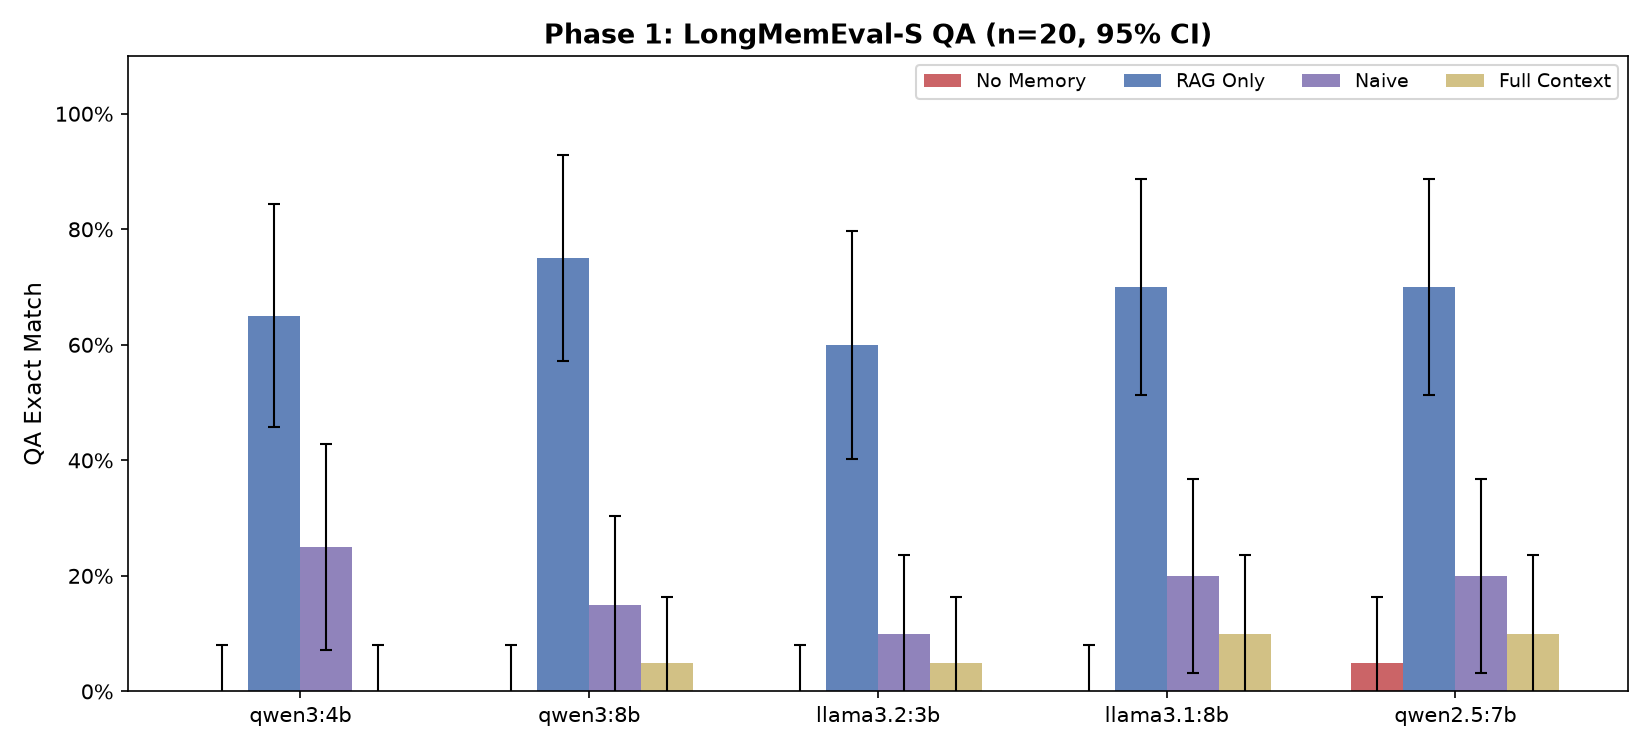
\includegraphics[width=\linewidth]{figures/fig5_phase1_qa.png}
  \caption{LongMemEval-S QA EM across all four conditions and five models.
    RAG Only consistently outperforms the Naive manager, confirming that
    memory rot actively degrades store quality below the raw-retrieval
    baseline.}
  \label{fig:phase1}
\end{figure}

\subsection{Phase 2: Memory Rot Characterization}
\label{sec:phase2}

Table~\ref{tab:ops} reports per-operation recall for the Naive and
Framework managers on the 80-turn injection stream.
Figures~\ref{fig:rotmean} and~\ref{fig:rot} show rot score accumulation
over turns.

\begin{figure}[t]
  \centering
  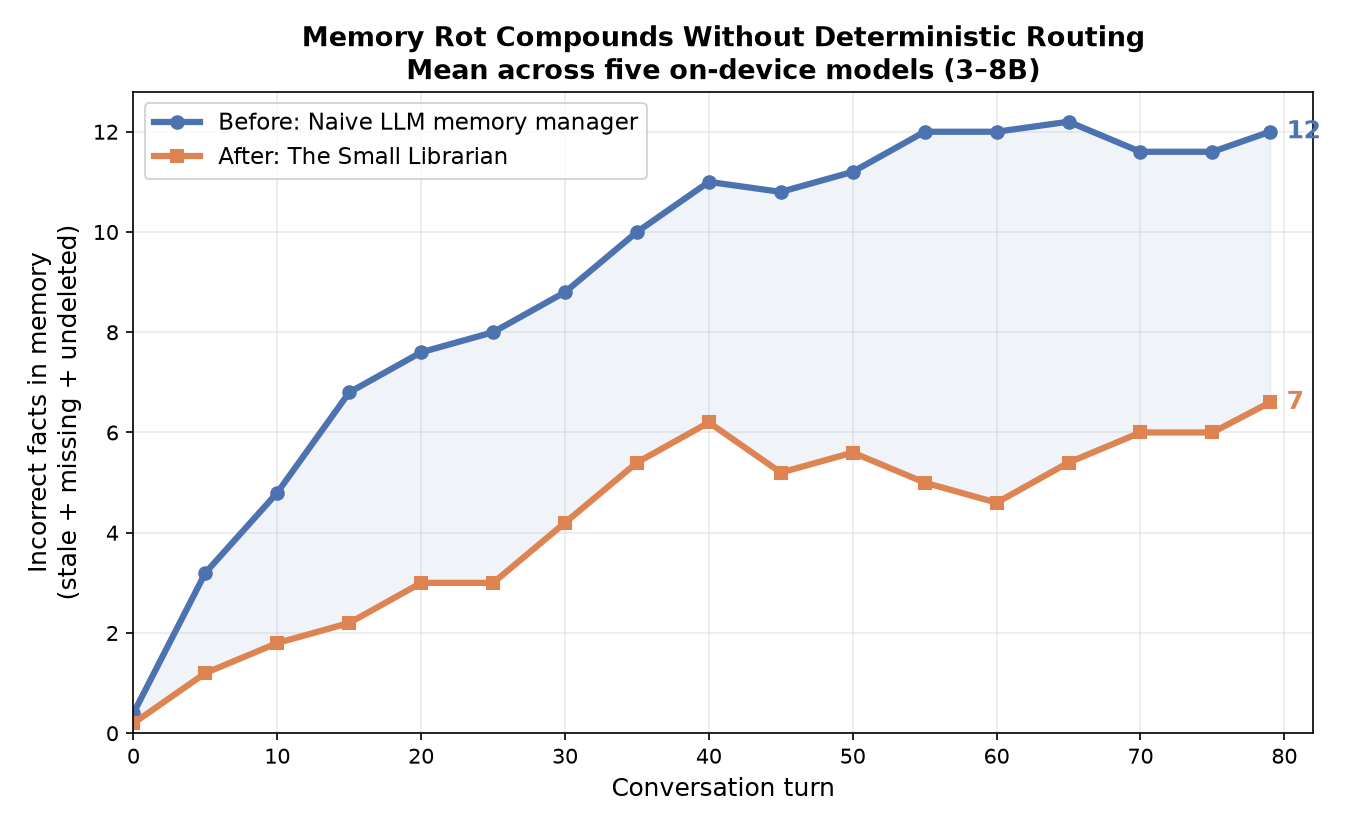
\includegraphics[width=\linewidth]{figures/fig8_rot_before_after.png}
  \caption{Memory rot compounds turn-over-turn without deterministic
    routing. Curves show the mean number of incorrect facts in memory
    (stale, missing, or undeleted) across all five on-device models.
    The Naive manager diverges from ground truth on $\sim$12 facts by
    turn~80; The Small Librarian holds at $\sim$7, roughly halving it.}
  \label{fig:rotmean}
\end{figure}

\paragraph{Near-zero UPDATE recall}
Under Naive, \textsc{update} recall is 0\% for three of five models.
Only LLaMA-3.1-8B shows partial capability (31\%), and even this is well
below what would be required for a reliable memory system.
The mean across all models is 10\%.

\paragraph{Bimodal NOOP collapse}
Two models (Qwen3-4B, Qwen2.5-7B) collapse entirely to \textsc{noop},
firing no operations regardless of turn content.
This is not a failure to understand the instructions but a mode collapse
under the combined pressure of long prompts and JSON-format constraints.
We verify this by inspecting raw model outputs: these models generate
``\texttt{\{"operations": [\{"op": "NOOP"\}]\}}'' for virtually every turn.

\paragraph{Framework improvements}
The Framework raises mean \textsc{update} recall from 10\% to 65\%.
The gains are consistent across all models except Qwen3-8B
(discussed in \S\ref{sec:anomaly}).
\textsc{delete} recall under the Framework (mean 26\%, matching Naive)
reflects the conservative keyword list design; precision rises dramatically
from 27\% (Naive) to 67\% (Framework).

\paragraph{Per-operation recall comparison}
Figures~\ref{fig:pernaive} and~\ref{fig:perfw} visualize the per-operation
recall profile for both managers across all five models.
The contrast is stark: the Naive manager is dominated by \textsc{add} and
\textsc{noop} bars, with \textsc{update} and \textsc{delete} nearly
invisible. The Framework inverts this pattern, achieving tall
\textsc{update} bars across all models while preserving meaningful
\textsc{add} recall.

\paragraph{Rot score accumulation}
Figure~\ref{fig:rotmean} shows the mean rot score across all five models,
and Figure~\ref{fig:rot} breaks it out per model.
Averaged across models, the Naive manager's memory diverges from ground
truth on 12 attributes by turn~80 and rises steadily, whereas the
Framework holds near 7, roughly halving the rot.
The gap is driven by the missing-fact term: models that collapse to
\textsc{noop} under Naive (Qwen3-4B, Qwen2.5-7B) leave the store empty and
therefore wrong about nearly every established fact (15 each by turn~80),
while the Framework writes those facts and stays at 5 and 10 respectively.
The pattern holds on four of five models; the sole exception is Qwen3-8B
(Naive~6, Framework~8), where the JSON-truncation artifact of
\S\ref{sec:anomaly} suppresses framework writes.
This corrects a naive reading in which an empty store appears
``rot-free'': an unwritten fact is not an absence of rot but a silent
error that surfaces the moment the fact is queried.

\begin{table}[t]
\centering
\caption{Per-operation recall (\%) on the 80-turn injection stream.
  Del.\ Prec.\ = \textsc{delete} precision for Framework.}
\label{tab:ops}
\setlength{\tabcolsep}{3pt}
\scriptsize
\begin{tabular}{lrrrr@{\hspace{6pt}}rrrr@{\hspace{6pt}}r}
\toprule
 & \multicolumn{4}{c}{\textbf{Naive Recall}} & \multicolumn{4}{c}{\textbf{Framework Recall}} & \textbf{Del.}\\
\textbf{Model} & AD & UP & DE & NO & AD & UP & DE & NO & \textbf{Prec.} \\
\midrule
Qwen3-4B     & 4  & 0  & 0  & 100 & 75  & 85 & 40 & 20  & 80\% \\
Qwen3-8B     & 96 & 12 & 40 & 0   & 42  & 23 & 20 & 80  & 100\% \\
LLaMA-3.2-3B & 54 & 8  & 40 & 0   & 58  & 92 & 20 & 0   & 40\% \\
LLaMA-3.1-8B & 12 & 31 & 50 & 0   & 71  & 88 & 40 & 0   & 80\% \\
Qwen2.5-7B   & 0  & 0  & 0  & 100 & 62  & 35 & 10 & 80  & 33\% \\
\midrule
\textit{Mean} & 33 & 10 & 26 & 40  & 62  & 65 & 26 & 36  & 67\% \\
\bottomrule
\end{tabular}
\end{table}

\begin{figure}[t]
  \centering
  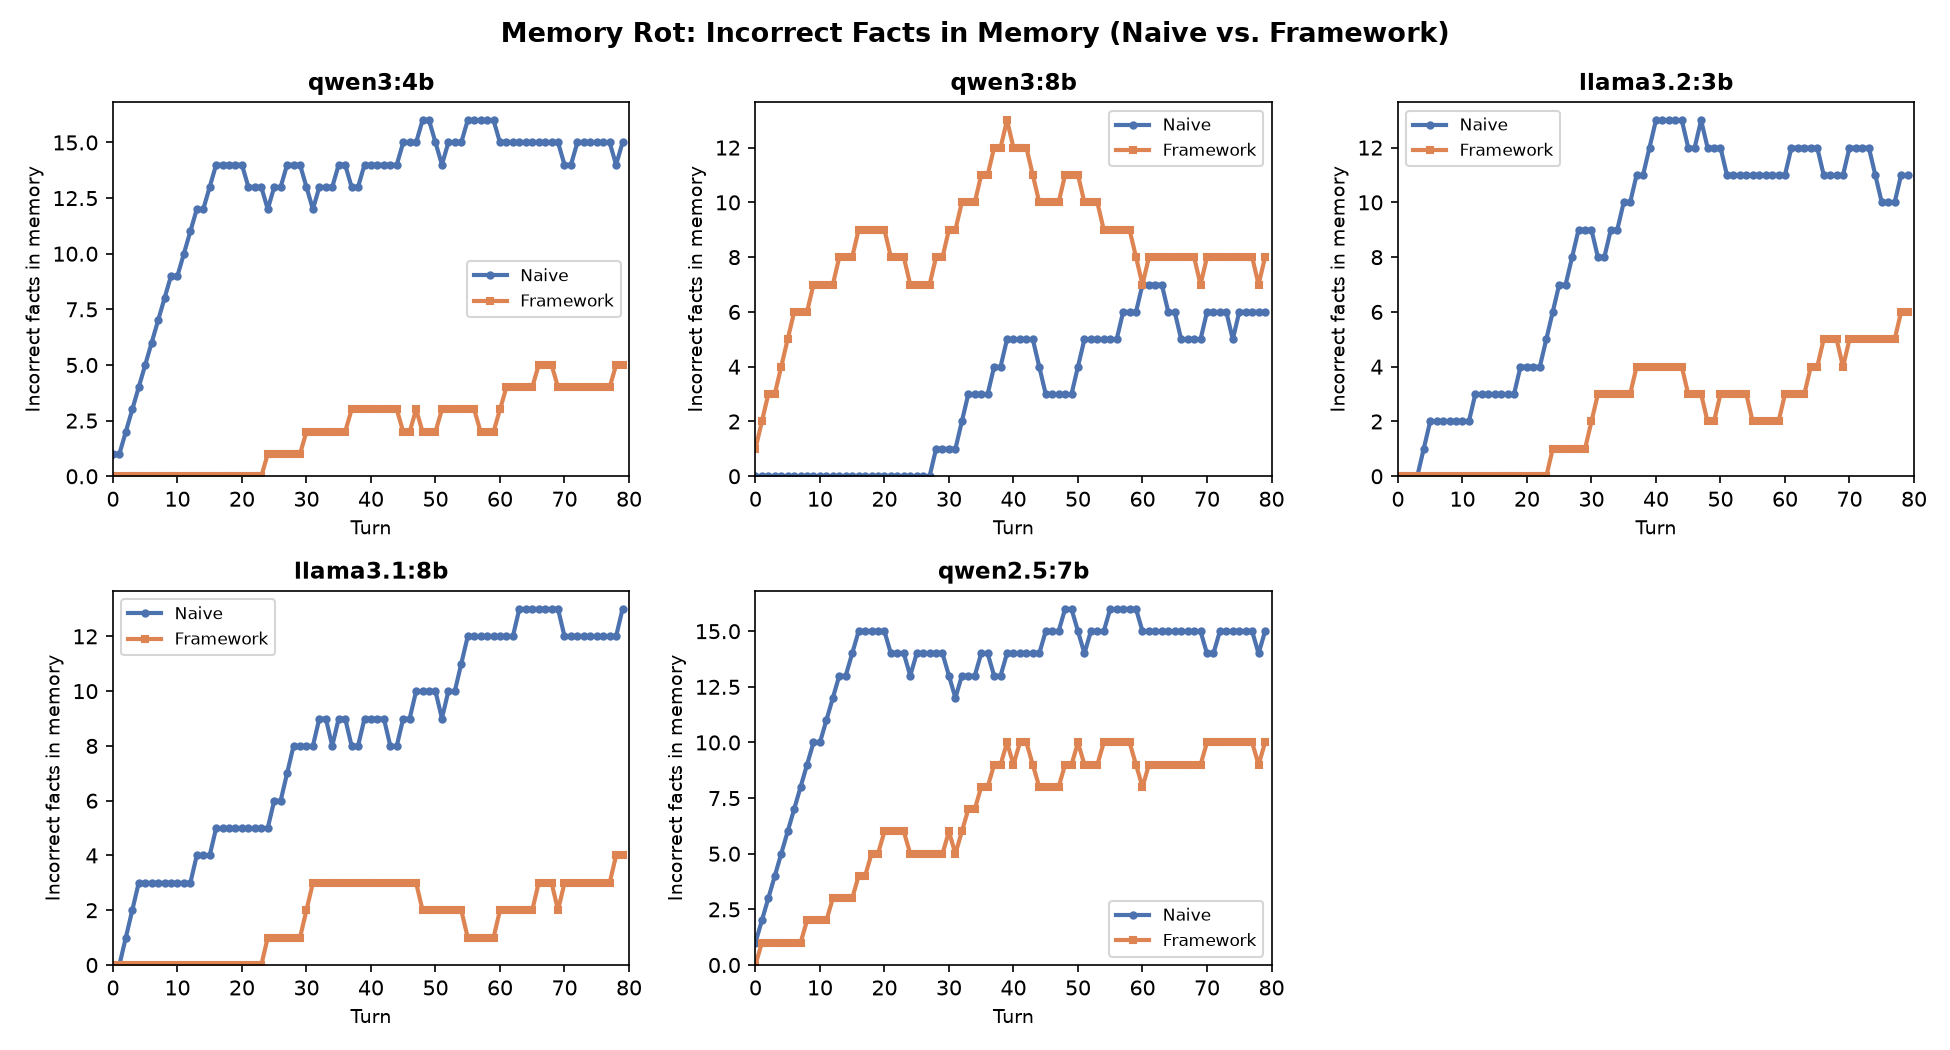
\includegraphics[width=\linewidth]{figures/fig4_rot_curves.png}
  \caption{Memory rot per model: incorrect facts in the store (stale +
    missing + undeleted) over turns, for Naive (blue) and Framework
    (orange). The Framework holds lower rot on four of five models.
    Qwen3-8B is the exception, where the JSON-truncation artifact
    (\S\ref{sec:anomaly}) suppresses framework writes.}
  \label{fig:rot}
\end{figure}

\begin{figure}[t]
  \centering
  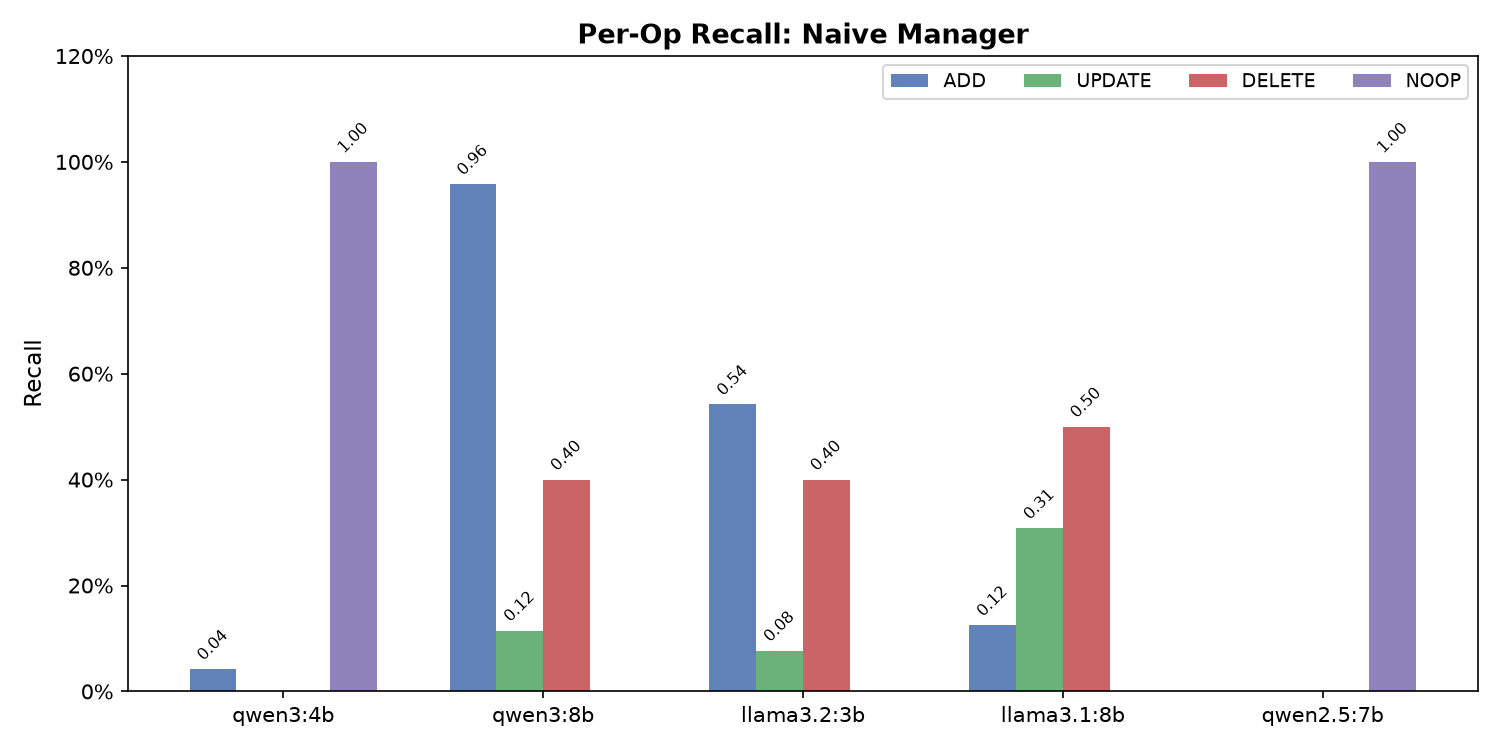
\includegraphics[width=\linewidth]{figures/fig2_per_op_naive.png}
  \caption{Per-operation recall under the Naive manager.
    \textsc{update} recall is near zero for all models; two models
    collapse entirely to \textsc{noop}. \textsc{add} absorbs most of
    the load where the model fires at all.}
  \label{fig:pernaive}
\end{figure}

\begin{figure}[t]
  \centering
  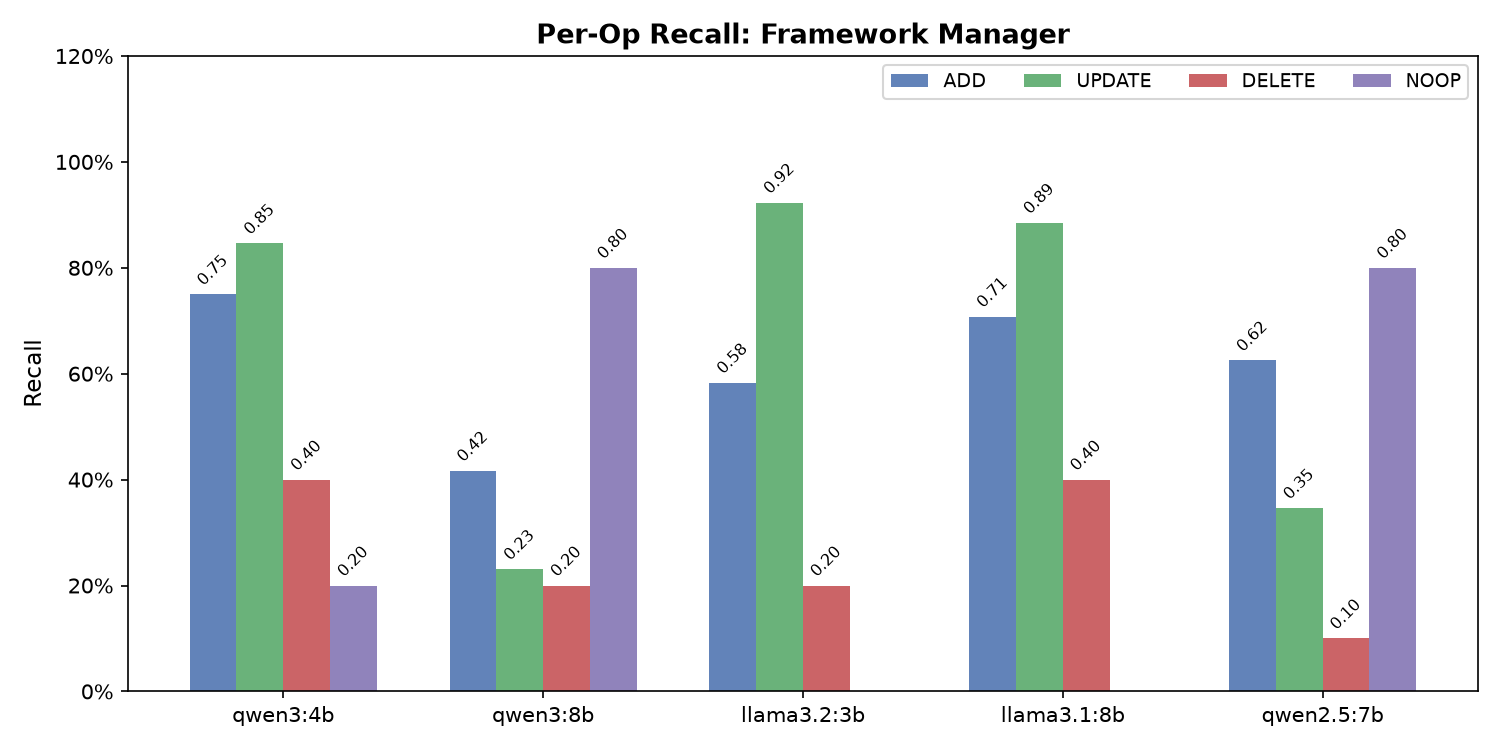
\includegraphics[width=\linewidth]{figures/fig3_per_op_fw.png}
  \caption{Per-operation recall under the Framework manager.
    \textsc{update} recall rises dramatically across all models.
    Comparing with Figure~\ref{fig:pernaive} shows that the Framework
    reshapes the operation distribution toward the correct ground truth.}
  \label{fig:perfw}
\end{figure}

\subsection{Ablation Study}
\label{sec:ablation}

Table~\ref{tab:ablation} reports \textsc{update} recall and QA EM across
four conditions on the injection stream QA set.
Figure~\ref{fig:ablation} visualizes \textsc{update} recall with 95\%
Wilson confidence intervals.

\paragraph{Typed slots dominate (UPDATE)}
The +Slots condition raises mean \textsc{update} recall from 10\% to
71\%, a 61 percentage-point gain.
For Qwen3-4B, the 95\% CI shifts from [0--13\%] to [71--96\%], fully
non-overlapping.
For LLaMA-3.2-3B the improvement is from 8\% to 100\% [87--100\%].
The typed slot mechanism requires no model changes, no additional training,
and no API calls beyond what is already used for fact extraction.

Crucially, typed slots also improve downstream QA EM: the mean injection-stream
QA EM rises from 41\% (Naive) to 60\% (+Slots).
This confirms that the \textsc{update} recall improvement translates to
better retrieval quality.

\paragraph{ADD recall remains stable}
The +Slots condition does not harm \textsc{add} recall: the mean stays at
62\% (Framework) vs.\ 33\% (Naive), with the Framework actually improving
\textsc{add} for models like Qwen3-4B (4\% to 75\%).
This is expected: typed slots only change how keys are written, not whether
new facts are ingested. Because the slot write always creates a new entry
when a key is absent, any fact the LLM extracts is stored, preserving or
improving \textsc{add} coverage.

\paragraph{Deletion signals: recall with precision tradeoff (DELETE)}
Adding deletion signals on top of typed slots (+Del) raises
\textsc{delete} recall (0\% to 10--40\%) and substantially improves
\textsc{delete} precision (see Figure~\ref{fig:delete}).
However, the QA EM mean is essentially unchanged (60\% to 59\%) because
two competing effects partially cancel:

\emph{Gains}: correctly deleting stale entries removes noise from retrieval.
\emph{Losses}: false-positive deletions erase correct entries.
For Qwen3-8B, two correct entries (city and car) are erroneously deleted,
dropping QA from 64\% to 50\%.

This tradeoff is model-dependent.
For Qwen3-4B, which had no \textsc{delete} capability at all under Naive,
deletion signals add net 8 percentage points of QA EM (71\% to 79\%) because
there are no false positives to erase.

\paragraph{NOOP and the precision cost of activity}
Under Naive, two models (Qwen3-4B and Qwen2.5-7B) collapse to
\textsc{noop} with 100\% recall, effectively refusing to write.
The Framework substantially reduces this rate (to 20\% and 80\%
respectively), converting those turns into productive \textsc{add} and
\textsc{update} operations.
For Qwen3-8B, the Framework increases \textsc{noop} rate from 0\% to 80\%
due to the JSON truncation artifact described in \S\ref{sec:anomaly}.

\paragraph{Compaction}
The +Compaction condition matches +Del across all models and metrics.
On the 80-turn stream with clean key normalization, no synonym-key
fragmentation accumulates, so compaction fires but finds nothing to merge.
Its benefit would become visible at longer horizons ($\geq$200 turns) or
with noisier key extraction, where users describe the same attribute with
varied phrasing across sessions.

\begin{table}[t]
\centering
\caption{4-condition ablation: \textsc{update} recall and QA EM.
  Nv=Naive, +Sl=+Typed Slots, +De=+Del.\ Signals, +Co=+Compaction. All \%.}
\label{tab:ablation}
\setlength{\tabcolsep}{3pt}
\small
\begin{tabular}{lrrrr@{\hspace{8pt}}rrrr}
\toprule
 & \multicolumn{4}{c}{\textbf{UPDATE Recall}} & \multicolumn{4}{c}{\textbf{QA EM}} \\
\textbf{Model} & Nv & +Sl & +De & +Co & Nv & +Sl & +De & +Co \\
\midrule
Qwen3-4B     & 0  & 88  & 85  & 81  & 29 & 71 & 79 & 79 \\
Qwen3-8B     & 12 & 27  & 23  & 23  & 64 & 64 & 50 & 50 \\
LLaMA-3.2-3B & 8  & 100 & 92  & 92  & 21 & 57 & 57 & 57 \\
LLaMA-3.1-8B & 31 & 96  & 88  & 88  & 64 & 50 & 50 & 50 \\
Qwen2.5-7B   & 0  & 46  & 35  & 35  & 29 & 57 & 57 & 57 \\
\midrule
\textit{Mean} & 10 & 71  & 65  & 64  & 41 & 60 & 59 & 59 \\
\bottomrule
\end{tabular}
\end{table}

\begin{figure}[t]
  \centering
  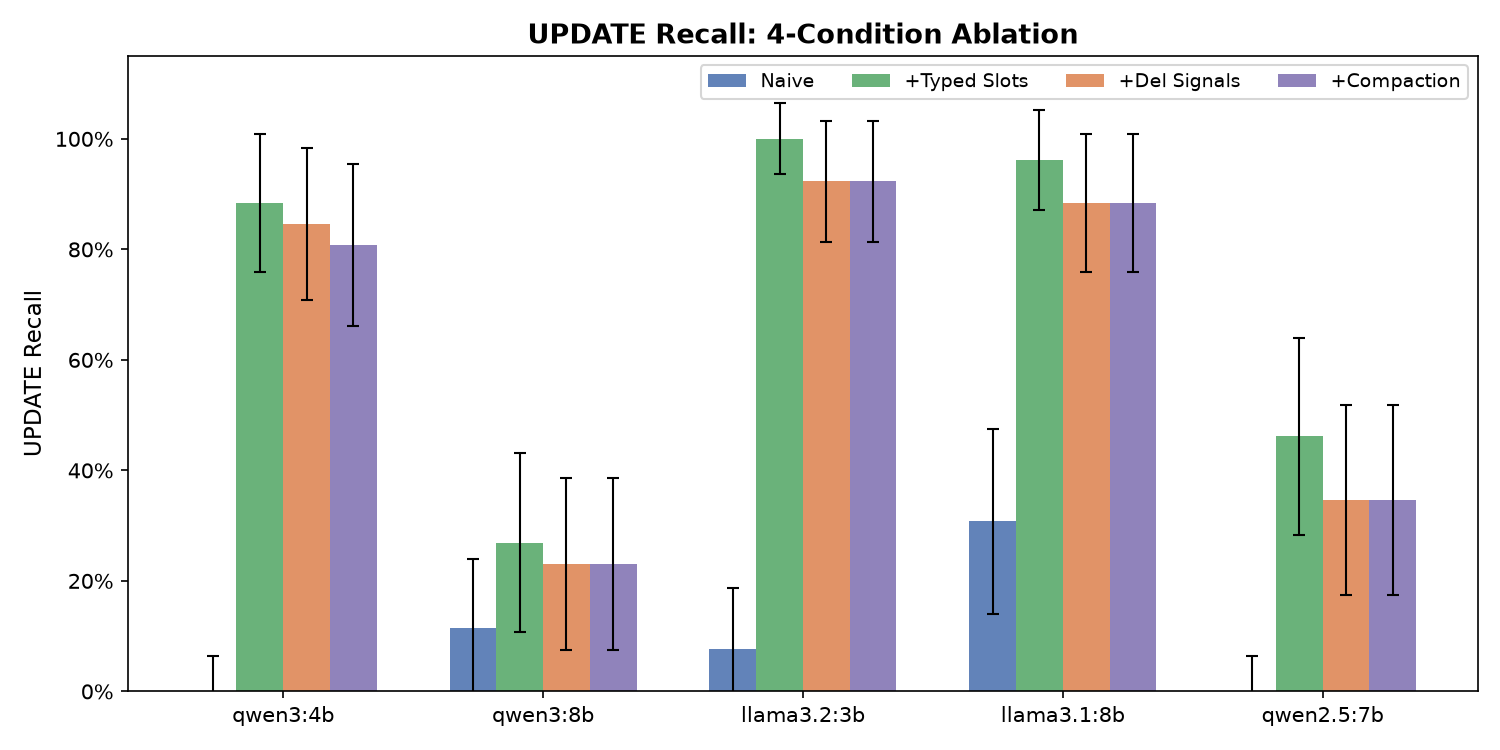
\includegraphics[width=\linewidth]{figures/fig1_ablation_update_recall.png}
  \caption{\textsc{update} recall across the 4-condition ablation with
    95\% Wilson CI error bars. Typed slots (+Slots) provide the dominant
    improvement for four of five models. Qwen3-8B is the persistent
    anomaly (\S\ref{sec:anomaly}).}
  \label{fig:ablation}
\end{figure}

%% ---------------------------------------------------------------------------------------------------------------------------------------------------------------------------------------------------------------------------------------
\section{Analysis}
\label{sec:analysis}

\subsection{Why RAG Outperforms Naive Memory Management}
\label{sec:rag_analysis}

The Phase~1 result (RAG $\gg$ Naive on LongMemEval-S) deserves careful
explanation, as it may seem counterintuitive: a structured memory store
should be more useful than raw retrieval.

The resolution is that memory rot makes the store \emph{less useful} than
the raw conversation.
When the Naive manager fires \textsc{noop} for most turns (Qwen3-4B and
Qwen2.5-7B), the store is nearly empty, missing most facts.
When it fires \textsc{add} indiscriminately (Qwen3-8B: 96\% \textsc{add}
recall), the store contains both current and superseded versions of facts.
In both cases, the store is a strictly worse signal source than the raw
conversation.

RAG sidesteps both failure modes: it retrieves the most recent mention of
any fact by recency-weighted similarity, which naturally surfaces updated
information.

This observation has an important practical implication: deploying an
LLM-managed store without validating operation-level recall may yield
\emph{worse outcomes than no structured memory at all}.
The Small Librarian framework restores the store's usefulness by ensuring
its write operations are reliable.

\subsection{The Qwen3-8B Anomaly}
\label{sec:anomaly}

Qwen3-8B stands out as an outlier: despite typed slots, its \textsc{update}
recall improves only modestly (from 12\% to 27\%), and it achieves the best
Phase~1 QA of any model under RAG (75\%) while showing the worst response to
the framework.

Inspection of raw model outputs reveals the root cause.
Qwen3-8B operates in a ``thinking'' mode under Ollama 0.32.x, generating
extensive chain-of-thought reasoning before producing the JSON response.
When the combined thinking and response tokens exceed the budget (800 tokens),
the JSON is truncated, producing an invalid response that our parser maps to
\textsc{noop}.
This explains both the high \textsc{noop} rate under the Framework (80\%) and
the weak \textsc{update} improvement.

This is an inference-stack artifact rather than a model capability limitation.
Under a different inference backend (or with a larger token budget), Qwen3-8B's
performance would likely match or exceed the other Qwen3 model.
We include it in our evaluation to accurately represent the real-world
on-device deployment experience, where inference quirks of this kind are common.

\subsection{The DELETE Precision--Recall Tradeoff}
\label{sec:delete_analysis}

Figure~\ref{fig:delete} plots \textsc{delete} recall against precision for
each condition across all models.
The Naive manager occupies a dispersed region with low precision (false
positives are common) and moderate recall.
Adding deletion signals moves points toward the upper-left quadrant:
higher precision, moderate recall.

The tradeoff reflects a deliberate design choice.
Our keyword list covers only \emph{explicit} negation.
Implicit deletions, where the user's statement implies a prior fact is
no longer true without using negation language, require semantic inference
that small models perform unreliably.
Extending to implicit deletions using an LLM classifier would trade the
precision benefit of rule-based detection for model-error risk.
We leave this as future work.

\begin{figure}[t]
  \centering
  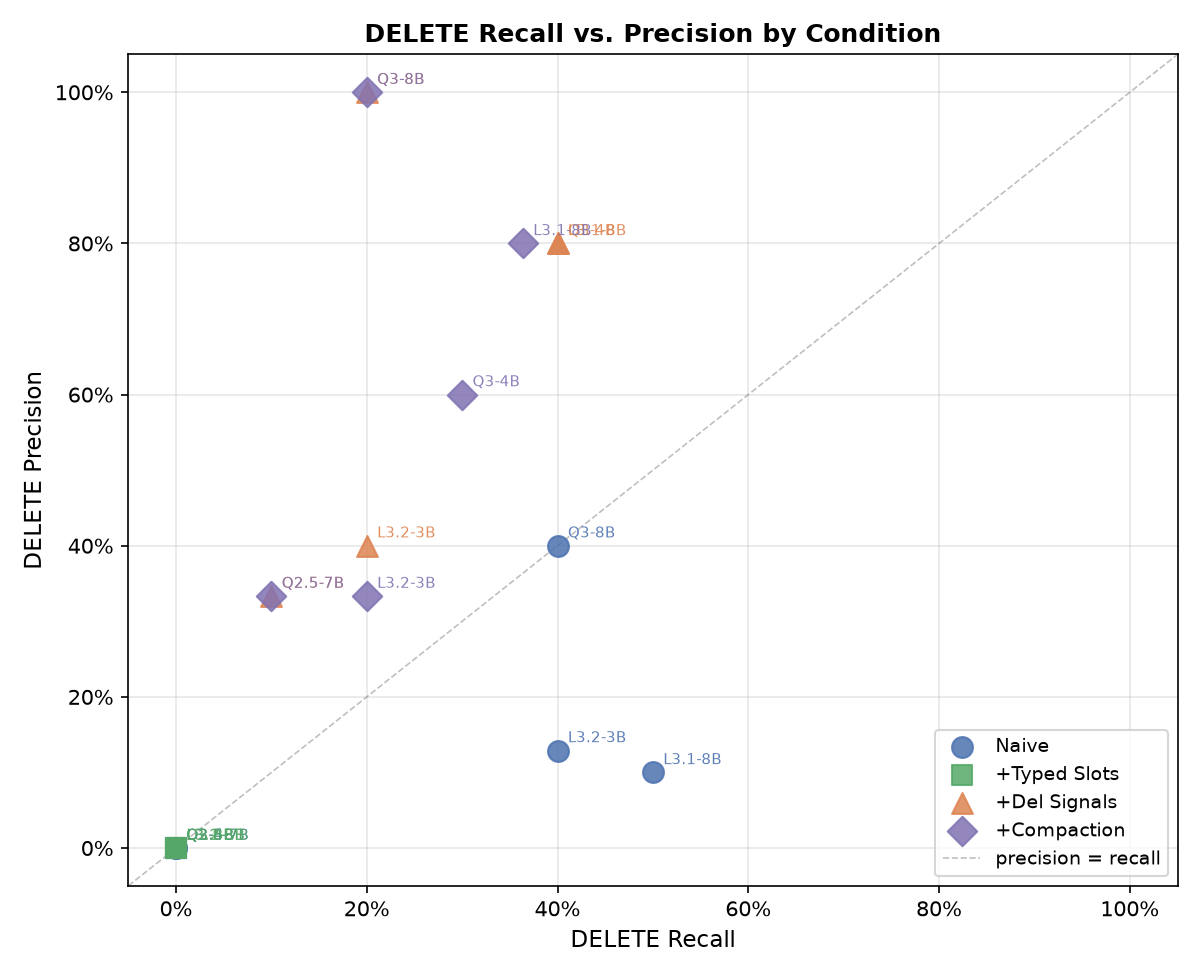
\includegraphics[width=\linewidth]{figures/fig6_delete_tradeoff.png}
  \caption{\textsc{delete} recall vs.\ precision by condition across all
    five models. Each point is annotated with its model identifier.
    Naive has low, variable precision. Deletion signals (triangles) and
    Compaction (diamonds) move points toward higher precision at moderate
    recall. The dashed line marks precision\,=\,recall.}
  \label{fig:delete}
\end{figure}

\subsection{QA--Operation Recall Decoupling}

A recurring pattern in our results is that QA EM and operation recall
do not always move together, for two reasons.

First, the QA evaluation on the injection stream covers all four operation
types, but the metric most sensitive to typed slots is
\textsc{update}-type questions (``What is the user's current X?'').
For these questions, typed slots consistently help.
\textsc{delete}-type questions (``Does the user still Y?'') benefit from
deletion signals but are also vulnerable to false-positive erasures.

Second, LongMemEval-S questions are drawn from real conversations, where the
most recent mention of a fact is often retrievable by RAG regardless of
store quality.
As a result, framework improvements on store quality do not uniformly
translate to Phase~1 QA gains; the RAG baseline is simply hard to beat
when the raw conversation contains the answer.

This decoupling is not just a measurement nuance; it has sharp practical
consequences for how AI systems with memory should be monitored and
evaluated. QA performance is a lagging indicator: a memory system can
suffer from severe operation-level rot for many turns before the rot
becomes visible in downstream answers. Two reasons explain the lag.
First, some QA questions happen to probe facts that were never updated or
deleted; for those questions, a rotten store and a healthy store give
identical answers. Second, retrieval systems have partial tolerance for
contradictions: when two versions of a fact coexist, the most recently
inserted one may still be retrieved first, masking the stale entry.
The net effect is that teams evaluating memory quality purely through
accuracy dashboards may observe healthy-looking numbers while the underlying
store silently accumulates stale entries that will eventually surface as
incorrect answers on the questions that matter most.

The correct diagnostic posture is to instrument memory operations
directly, tracking per-operation recall and precision in parallel with
downstream QA. A system that shows high QA EM but low \textsc{update}
recall is not functioning correctly; it is benefiting from retrieval
tolerance of a problem that will compound over time. Conversely, a
system that shows near-perfect \textsc{update} and \textsc{delete}
recall provides a much stronger guarantee of correctness even if its
instantaneous QA score is similar to a rotten store.
Operation-level metrics are the only way to distinguish these two regimes.

%% ---------------------------------------------------------------------------------------------------------------------------------------------------------------------------------------------------------------------------------------
\section{Limitations}
\label{sec:limitations}

\paragraph{Sample size}
All Phase~1 conditions use $n=20$ LongMemEval-S examples.
The resulting 95\% Wilson confidence intervals span $\pm$15--22 percentage
points.
Results should be interpreted as directional.
The \textsc{update} recall improvements for typed slots (61~pp mean gain)
are large enough to be unambiguous, but finer distinctions, such as whether
deletion signals help or hurt net QA, require replication at $n \geq 50$.

\paragraph{Synthetic injection stream}
The controlled stream uses authored turns with intentionally clean key
normalization, making extraction easier than in real conversations.
Real user turns express the same attribute with greater variety
(\emph{``My new car is a BMW''} vs.\ \emph{``Bought a BMW X5 last week''}).
This would increase key extraction noise and compaction's importance.

\paragraph{Single benchmark}
We evaluate downstream QA on LongMemEval-S only.
A second benchmark (e.g., LoCoMo~\cite{maharana2024evaluating}) would
strengthen generalizability.
We treat this as the highest-priority extension.

\paragraph{Qwen3 thinking mode}
Qwen3 models under Ollama 0.32.x route structured JSON output to an
internal thinking field, requiring a fallback heuristic that truncates
the thinking chain and reads its last line.
This may underestimate Qwen3 framework performance; we include it to
accurately reflect real on-device deployment conditions.

\paragraph{Token budget sensitivity}
Several of our findings (the Qwen3-8B anomaly, NOOP collapse in Qwen3-4B
and Qwen2.5-7B) are sensitive to the token generation budget and prompt
format.
A more thorough prompt engineering sweep might recover additional performance
from these models.

%% ---------------------------------------------------------------------------------------------------------------------------------------------------------------------------------------------------------------------------------------
\section{Conclusion}
\label{sec:conclusion}

We introduced \emph{memory rot}, the near-complete failure of small
on-device models to fire \textsc{update} and \textsc{delete} memory
operations, and proposed The Small Librarian framework to repair it.

The diagnosis is clear: naive LLM-driven memory management achieves only
10\% mean \textsc{update} recall across five models, causing memory stores to
accumulate contradictions that degrade retrieval below even the RAG baseline.
The remedy is equally clear: replace the probabilistic routing decision with
deterministic mechanisms.
Typed slots raise mean \textsc{update} recall to 71\% with no additional
parameters or API calls.
Deletion signals extend the framework to \textsc{delete}, revealing a
precision--recall tradeoff that motivates compaction for longer-horizon
deployments.

More broadly, this work demonstrates that memory management quality cannot
be safely inferred from downstream QA alone.
RAG over raw turns outperforms a naive LLM-managed store, not because
retrieval is inherently superior, but because memory rot makes the store
less trustworthy than the raw conversation.
Fixing the store, making its write operations reliable, is necessary
before structured memory can realize its potential advantage over RAG.

The Small Librarian is one step in that direction: it keeps the LLM in
the loop only for what it does reliably (extracting facts from natural
language), and handles routing deterministically where models consistently
fail.
We believe this principle, \emph{deterministic where possible and learned
where necessary}, is a productive design philosophy for building reliable
memory systems from unreliable small models.

%% ---------------------------------------------------------------------------------------------------------------------------------------------------------------------------------------------------------------------------------------
\section*{Acknowledgements}

All experiments were conducted on a consumer Apple M-series laptop using
open-weight models served locally via Ollama.
No cloud GPU resources or paid API credits were used in the primary
experiments.

%% ---------------------------------------------------------------------------------------------------------------------------------------------------------------------------------------------------------------------------------------
\section*{Practical Implications for Memory-Augmented AI Systems}
\label{sec:implications}

The failure modes described in this paper are not unique to small on-device
models. Any LLM-driven memory system that relies on the model to choose
between \textsc{add}, \textsc{update}, and \textsc{delete} is exposed to
memory rot. Larger frontier models reduce the severity, but the routing
problem does not disappear: models with limited context awareness, long
system prompts, or schema-heavy output constraints can exhibit the same
systematic \textsc{add} bias we document here.
The following design principles are extracted from our results and apply
to memory architectures at any scale.

\paragraph{Prefer deterministic routing over model judgment}
The central lesson of this work is that the \textsc{update}/\textsc{delete}
routing decision is better handled by the system than by the model.
When a fact key can be normalized to a canonical form, the system knows
whether that key already exists and can execute the correct operation
without asking the model to choose.
Typed slots operationalize this for on-device models, but the principle
extends to any architecture: define a schema, maintain a keyspace, and
use key presence to route writes deterministically.
Even with large models, adding this layer reduces error rates and makes
behavior auditable.

\paragraph{Measure operations, not just outcomes}
QA accuracy is a necessary but insufficient signal for memory health.
Teams building conversational AI systems should instrument per-operation
recall and precision alongside task accuracy, and monitor them continuously.
A system that shows stable QA accuracy while \textsc{update} recall
is declining is accumulating hidden rot that will eventually surface as
incorrect answers. Establish baseline operation-level metrics before
deployment and set alert thresholds on degradation.

\paragraph{Design the memory schema before the prompt}
Memory rot is harder to introduce when the memory schema is explicit and
stable. Define what attributes the agent tracks (a keyspace), normalize
how those attributes are named, and ensure the extraction prompt returns
structured key-value pairs tied to that schema. This separates extraction
(what the fact is) from routing (whether it is new), letting the system
handle the latter deterministically. Unstructured free-text stores
maximize model flexibility but eliminate the possibility of deterministic
routing.

\paragraph{Use keyword deletion signals as a first-pass filter}
For any class of facts that users revoke using predictable language (job
changes, relationship updates, discontinued habits), a curated keyword
list provides high-precision deletion triggers at zero model cost.
The precision advantage of rule-based signals over LLM-based DELETE
routing is consistent across all models we tested. In production, such
a list can be maintained by the application team and updated as patterns
emerge from user logs. Reserve LLM-based semantic inference for the
harder, linguistically implicit deletions that keywords cannot catch.

\paragraph{Compact the store periodically}
Any memory system that relies on key normalization will accumulate synonym
fragmentation over long horizons. Periodic compaction, driven by an LLM
that identifies semantically equivalent keys, prevents the store from
bifurcating facts that belong together.
The compaction cadence should be calibrated to the rate of synonym
accumulation; in our 80-turn experiments no compaction was needed, but
real deployments spanning months of interaction will require it.

\paragraph{Apply these principles beyond memory management}
The broader principle, deterministic where possible and learned where
necessary, applies to any agentic pipeline with structured side effects.
Tool routing, database writes, and API calls all benefit from the same
separation: let the LLM extract intent and parameters, and let the system
decide \emph{which} operation to execute based on known state.
Wherever a model's output triggers a side effect that is difficult to
reverse, inserting a deterministic routing layer reduces the blast radius
of model errors and makes the system's behavior predictable and auditable.

%% ---------------------------------------------------------------------------------------------------------------------------------------------------------------------------------------------------------------------------------------
\bibliographystyle{abbrvnat}
\bibliography{refs}

\end{document}
